\documentclass[a4paper,portrait]{article}
\usepackage{amssymb}
\usepackage[utf8]{inputenc}
\usepackage[T1]{fontenc}
\usepackage{lmodern}
\usepackage{geometry}
\usepackage{multicol}
\usepackage{titlesec}
\usepackage{xcolor}
\usepackage{graphicx}
\usepackage{hyperref}
\usepackage{array}
\usepackage{amsmath}

% Geometry for landscape layout
\geometry{left=1.5cm, right=1.5cm, top=1.5cm, bottom=1.5cm}

% Custom colors
\definecolor{titlecolor}{RGB}{0, 102, 204}
\definecolor{sectioncolor}{RGB}{51, 51, 51}
\definecolor{subsectioncolor}{RGB}{51, 51, 51}

% Title formatting
\titleformat{\section}
{\normalfont\Large\bfseries\color{titlecolor}}
{\thesection}{1em}{}

\titleformat{\subsection}
{\normalfont\large\bfseries\color{sectioncolor}}
{\thesubsection}{1em}{}

% Add vertical rules between columns
\setlength{\columnsep}{20pt}
\setlength{\columnseprule}{0.4pt}
\def\columnseprulecolor{\color{gray}}

\begin{document}

% Multicols environment
\begin{multicols}{2}
\setlength\columnsep{20pt} % Space between columns

\begin{center}
    \huge\textbf{APprentissage STAtistique}\\
     2024-2025
\end{center}

% Section 1: Introduction
\section*{Introduction}
L'intelligence artificielle (IA) représente la théorie et le développement de systèmes informatiques capables d'effectuer des tâches nécessitant normalement l'intelligence humaine. 

\textbf{\\} L’apprentissage automatique, c’est la capacité d’un ordinateur à apprendre sans avoir été explicitement programmé.
 
\subsection{Exemple d'un modèle supervisé :}

\begin{center}
    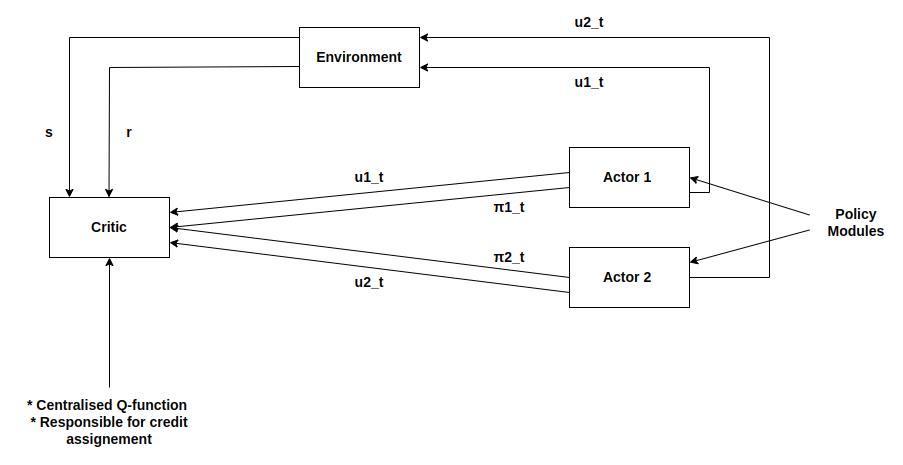
\includegraphics[width=0.9\linewidth]{1.png}
\end{center}

\subsection{La fonction de risque dans l'apprentissage :}

\begin{center}
    
\includegraphics[width=1\linewidth]{image.jpg}

\end{center}
    
Idéalement :   \[
f^*_{Bayes} = \arg\min_{f \in \mathcal{F}_{all}} R(f)
\]
\[
R(f) = \int L(y, f(x)) dP(x, y)
\]

Mais \( f \) est un certain type de fonction :  
\[
f^* = \arg\min_{f \in \mathcal{F}} R(f)
\]

Cependant, nous n'avons pas accès à la distribution :  
\[
\hat{f}_{erm} = \arg\min_{f \in \mathcal{F}} R_{erm}(f)
\]
\[
R_{erm}(f) = \frac{1}{N} \sum_{i=1}^N L(y, f(x))
\]

\subsection{Décomposition biais-variance :}
\[
\mathbb{E}\left[(\hat{y} - y)^2\right] = \mathbb{E}\left[(\hat{y} - \mathbb{E}[\hat{y}] + \mathbb{E}[\hat{y}] - y)^2\right]
\]
\[
= \mathbb{E}\left[(\hat{y} - \mathbb{E}[\hat{y}])^2 + 2(\hat{y} - \mathbb{E}[\hat{y}])(\mathbb{E}[\hat{y}] - y) + (\mathbb{E}[\hat{y}] - y)^2\right]
\]
\[
= \mathbb{E}\left[(\hat{y} - \mathbb{E}[\hat{y}])^2\right] + \mathbb{E}\left[2(\hat{y} - \mathbb{E}[\hat{y}])(\mathbb{E}[\hat{y}] - y)\right] + \mathbb{E}\left[(\mathbb{E}[\hat{y}] - y)^2\right]
\]
\[
= \mathbb{E}\left[(\hat{y} - \mathbb{E}[\hat{y}])^2\right] + 2(\mathbb{E}[\hat{y}] - y)\mathbb{E}\left[(\hat{y} - \mathbb{E}[\hat{y}])\right] + (\mathbb{E}[\hat{y}] - y)^2
\]
\[
= \mathbb{E}\left[(\hat{y} - \mathbb{E}[\hat{y}])^2\right] + (\mathbb{E}[\hat{y}] - y)^2
\]
\[
= \mathrm{var}(\hat{y}) + \mathrm{bias}(\hat{y}, y)^2
\]

\subsection{Dataset split}
\begin{itemize}
    \item Ensemble d'entraînement : pour adapter les paramètres du modèle.
    \item Ensemble de validation : pour ajuster la complexité du modèle.
    \item Ensemble de test : pour évaluer la performance du modèle.
\end{itemize}

% Section 2: Méthodes principales
\section{Méthodes principales}

\subsection{Apprentissage supervisé}
Utilisé pour des données étiquetées, où l'objectif est de prédire \(y\) à partir de \(x\). Il peut être divisé en :

\begin{itemize}
    \item \textbf{Régression}: prédiction de valeurs continues.
    \item \textbf{Classification}: attribution de labels à des exemples.
\end{itemize}

\subsection{Apprentissage non supervisé}
Utilisé pour découvrir des structures dans des données non étiquetées, comprenant :

\begin{itemize}
    \item \textbf{Clustering}:  regroupement de données similaires.
    \item \textbf{Réduction de dimension}: élimination des caractéristiques non pertinentes.
\end{itemize}

\subsection{Apprentissage par renforcement}
Basé sur un agent qui interagit avec un environnement pour maximiser une récompense cumulative, souvent à travers le Q-learning ou les DNN.

% Explications détaillées des algorithmes

\subsection{Autres classifications}

\textbf{Par nature :}
\begin{itemize}
    \item \textbf{Symbolistes} : Règles et arbres de décision
    \item \textbf{Bayésiens} : Naive Bayes ou Markov
    \item \textbf{Connectionnistes} : Réseaux neuronaux
    \item \textbf{Évolutionnistes} : Programmes génétiques
    \item \textbf{Analogistes} : Vecteurs de support
\end{itemize}

\textbf{\\Par Taxonomie :}

\begin{itemize}
    \item \textbf{Discriminatif vs Génératif} :
    \begin{itemize}
        \item Modèles spécialisés pour distinguer (discriminatif).
        \item Modèles capables d'expliquer comment générer de nouvelles données (génératif).
    \end{itemize}
    
    \item \textbf{Basé instance vs. Basé modèle} :
    \begin{itemize}
        \item On stocke les données d'entraînement (e.g., K-NN, SVM).
        \item On résume les données avec un modèle (e.g., modèles paramétriques).
    \end{itemize}
\end{itemize}

\section{Régression}

\subsection{Régression linéaire}

\textbf{Objectif} : Trouver une fonction linéaire \( y = \mathbf{w}^T \mathbf{x} + b \) qui minimise l'erreur quadratique entre les valeurs observées \( y_i \) et les prédictions \( \hat{y}_i \).

\textbf{Formulation} :
\[
L_{\text{SE}} = \frac{1}{N} \sum_{i=1}^{N} \left( y_i - \left(\mathbf{w}^T \mathbf{x}_i + b \right)\right)^2
\]
où \( \mathbf{w} \) est le vecteur des coefficients, et \( b \) est le biais. La solution analytique est donnée par la formule des moindres carrés :
\[
\mathbf{w} = (\mathbf{X}^T \mathbf{X})^{-1} \mathbf{X}^T \mathbf{y}
\]


\textbf{Points forts} : Facile à comprendre et rapide pour des petites dimensions.

\textbf{Points faibles} : Sensible aux valeurs aberrantes et nécessite des données linéaires.

\subsection{Régression Ridge/Lasso}
Le modèle peut être régularisé avec les méthodes Ridge ($\ell_2$) ou Lasso ($\ell_2$) pour éviter l'overfitting :
\[
L_{\text{Ridge}} = L_{\text{SE}} + \lambda \|\mathbf{w}\|_2, \quad L_{\text{Lasso}} = L_{\text{SE}} + \lambda \|\mathbf{w}\|_1
\]


La pénalisation $\ell_1$ favorise la parcimonie alors que $\ell_2$ favorise la dérivabilité.

\textbf{\\Démonstration KRR}

\subsection*{1. Transformer la fonction de perte}
La fonction de perte pour la régression ridge à noyau (KRR) est :
\[
L(w) = \frac{1}{2} \| y - \Phi w \|^2 + \frac{\lambda}{2} \| w \|^2
\]
On substitue \( w = \sum_{i=1}^{n} a_i \phi(x_i) = \Phi^T a \) :
\[
L(a) = \frac{1}{2} \| y - K a \|^2 + \frac{\lambda}{2} a^T K a
\]
où \( K = \Phi \Phi^T \) et \( K_{ij} = k(x_i, x_j) \).

\subsection*{2. Dériver et résoudre pour \( a \)}
On prend la dérivée de \( L(a) \) :
\[
\frac{\partial L(a)}{\partial a} = -K^T (y - K a) + \lambda K a
\]
On annule la dérivée :
\[
K y = K (K + \lambda I) a
\]
En supposant \( K \) inversible :
\[
a = (K + \lambda I)^{-1} y
\]

\subsection*{3. Prédire pour un nouveau point \( x_{\text{new}} \)}
La prédiction est :
\[
f(x_{\text{new}}) = \sum_{i=1}^{n} a_i k(x_i, x_{\text{new}})
\]
Sous forme matricielle :
\[
f(x_{\text{new}}) = k_{\text{new}}^T a
\]
où \( k_{\text{new}} = [k(x_1, x_{\text{new}}), \dots, k(x_n, x_{\text{new}})]^T \).

\subsection*{4. KRR vs SVM}
\subsubsection*{Similitudes :}
\begin{itemize}
    \item Les deux utilisent l'astuce du noyau pour modéliser des relations non linéaires.
    \item Les deux intègrent une régularisation.
    \item Les deux reposent sur des formulations duales.
\end{itemize}

\subsubsection*{Différences :}
\begin{itemize}
    \item KRR minimise l'erreur quadratique ; SVM minimise la perte hinge.
    \item Les solutions SVM sont parcimonieuses ; les solutions KRR ne le sont pas.
    \item SVM a une interprétation géométrique (maximisation de la marge) ; KRR n'en a pas.
\end{itemize}


\newpage

\section{Classification}
\subsection{Régression logistique}

\textbf{Objectif} : Modéliser la probabilité qu'une observation \( x \) appartienne à la classe \( y = 1 \) via la fonction sigmoïde :
\[
P(y = 1 | x) = \sigma(\mathbf{w}^Tx)=\frac{1}{1 + e^{-(\mathbf{w}^T \mathbf{x} + b)}}
\]

\textbf{Fondement} : La régression logistique repose sur la distribution de Bernoulli pour modéliser la probabilité de la classe positive :
\[
P(y \mid \mathbf{x}) = \sigma(\mathbf{w}^T \mathbf{x})^y (1 - \sigma(\mathbf{w}^T \mathbf{x}))^{1-y}
\]
La fonction de coût à minimiser est la log-vraisemblance négative (ou cross-entropy) :
\[
L_{\text{CE}} = - \frac{1}{N} \sum_{i=1}^{N} \left( y_i \log(\hat{y}_i) + (1 - y_i) \log(1 - \hat{y}_i) \right)
\]

\textbf{Solution} : Utilisation de la descente de gradient pour minimiser cette fonction de coût.

\textbf{Points forts} : probabiliste, coût calculatoire faible, facile à implémenter, entraîner et interpréter.

\textbf{Points faibles} : Ne gère pas bien les relations non-linéaires, nécessite de bonnes features.

\textbf{Extension aux dimensions supérieures} : on étend sigmoid à SoftMax et cross-entropy à categorical cross entropy :

\[P(y = k | \mathbf{x}) = \frac{e^{z_k}}{\sum_{j=1}^K e^{z_j}}\]

\[L_{\text{CE}} = - \sum_{i=1}^N \sum_{k=1}^K 1_{\{y_i = k\}} \log(P(y_i = k | \mathbf{x}_i))\]

\textbf{Log-Odds Ratio (réciproque de sigmoid) : }
\[
\text{logit}(P(y=1 \mid \mathbf{x})) = \ln\left(\frac{P(y=1 \mid \mathbf{x})}{P(y=0 \mid \mathbf{x})}\right)
\]

\begin{itemize}
    \item \( w_i > 0 \) : Les cotes augmentent.
    \item \( w_i < 0 \) : Les cotes diminuent.
    \item \( w_i = 0 \) : Les cotes restent inchangées.
\end{itemize}

Cette interprétation est particulièrement utile pour évaluer l'influence des caractéristiques.

\subsection{K-Nearest Neighbors (KNN)}
Soit un point de données \( x \) et un ensemble d'entraînement \( \{(x_i, y_i)\}_{i=1}^n \). Pour prédire la classe ou la valeur de \( x \) :
\begin{enumerate}
    \item Calculer les distances \( d(x, x_i) \) (e.g., distance euclidienne).
    \item Sélectionner les \( k \) plus proches voisins \( \mathcal{N}_k(x) \).
    \item Pour la classification : 
        \[
        \hat{y} = \text{mode}(\{y_i \mid x_i \in \mathcal{N}_k(x)\})
        \]
    \item Pour la régression :
        \[
        \hat{y} = \frac{1}{k} \sum_{x_i \in \mathcal{N}_k(x)} y_i
        \]
\end{enumerate}

\textbf{Avantages :}
\begin{itemize}
    \item Solution multi-classes réelle.
    \item Classificateur intuitif.
    \item L'entraînement consiste uniquement à stocker l'ensemble d'entraînement.
    \item Flexibilité dans le choix du voisinage et de la distance.
\end{itemize}

\textbf{Inconvénients :}
\begin{itemize}
    \item Besoin en mémoire important.
    \item Coût computationnel élevé.
\end{itemize}

\subsection{Support Vector Machines (SVM)}

\textbf{Objectif} : Trouver un hyperplan optimal qui sépare deux classes en maximisant la marge entre les points les plus proches (vecteurs de support). Pour des données non linéairement séparables, une marge souple (soft margin) est introduite pour tolérer les erreurs de classification.

\subsubsection{Hyperplan séparateur optimal}

\textbf{Problème} : Maximiser la marge \( \frac{1}{\|\mathbf{w}\|} \) tout en classant correctement les données :
\[
\min_{\mathbf{w}, w_0} \frac{1}{2} \|\mathbf{w}\|^2 \quad \text{sous} \quad y_i (\mathbf{w}^T \mathbf{x}_i + w_0) \geq 1 \quad \forall i
\]

\textbf{Formulation duale} : Le problème est reformulé en termes de multiplicateurs de Lagrange \( \alpha_i \) :
\[
\max_{\alpha} \sum_{i=1}^n \alpha_i - \frac{1}{2} \sum_{i,j=1}^n \alpha_i \alpha_j y_i y_j \mathbf{x}_i^T \mathbf{x}_j
\]
sous les contraintes :
\[
\sum_{i=1}^n \alpha_i y_i = 0 \quad \text{et} \quad \alpha_i \geq 0 \quad \forall i
\]

\textbf{Vecteurs de support} : Seuls les points avec \( \alpha_i > 0 \) (vecteurs de support) contribuent à la solution :
\[
\mathbf{w} = \sum_{i=1}^n \alpha_i y_i \mathbf{x}_i \quad \text{et} \quad w_0 = y_{\text{SV}} - \mathbf{w}^T \mathbf{x}_{\text{SV}}
\]


\subsubsection{Marge souple (Soft Margin)}

Pour les données non séparables, des variables de relaxation \( \xi_i \) sont introduites :
\[
\min_{\mathbf{w}, w_0, \xi} \frac{1}{2} \|\mathbf{w}\|^2 + C \sum_{i=1}^n \xi_i
\]
sous les contraintes :
\[
y_i (\mathbf{w}^T \mathbf{x}_i + w_0) \geq 1 - \xi_i \quad \text{et} \quad \xi_i \geq 0 \quad \forall i
\]
où \( C \) contrôle le compromis entre la marge et les erreurs.

\subsubsection{Kernel Trick}

Pour les données non linéairement séparables, les données sont projetées dans un espace de grande dimension via une fonction \( \phi(\mathbf{x}) \). Le produit scalaire \( \phi(\mathbf{x}_i)^T \phi(\mathbf{x}_j) \) est remplacé par un noyau \( K(\mathbf{x}_i, \mathbf{x}_j) \).
\\\\
\textbf{Formulation duale avec noyau} :
\[
\max_{\alpha} \sum_{i=1}^n \alpha_i - \frac{1}{2} \sum_{i,j=1}^n \alpha_i \alpha_j y_i y_j K(\mathbf{x}_i, \mathbf{x}_j)
\]
sous les mêmes contraintes que précédemment.
\\\\
\textbf{Exemples de noyaux} :
\begin{itemize}
    \item Linéaire : \( K(\mathbf{x}_i, \mathbf{x}_j) = \mathbf{x}_i^T \mathbf{x}_j \)
    \item Polynomial : \( K(\mathbf{x}_i, \mathbf{x}_j) = (1 + \mathbf{x}_i^T \mathbf{x}_j)^d \)
    \item RBF : \( K(\mathbf{x}_i, \mathbf{x}_j) = \exp(-\gamma \|\mathbf{x}_i - \mathbf{x}_j\|^2) \)
\end{itemize}

\subsubsection{Prédiction}

Pour un nouveau point \( \mathbf{x}_{\text{new}} \), la décision est donnée par :
\[
f(\mathbf{x}_{\text{new}}) = \text{sign}\left( \sum_{i=1}^n \alpha_i y_i K(\mathbf{x}_i, \mathbf{x}_{\text{new}}) + w_0 \right)
\]


\subsubsection{Points forts et faibles}

\textbf{Points forts} :
\begin{itemize}
    \item Efficace pour les données linéairement et non linéairement séparables.
    \item Généralisation robuste grâce à la maximisation de la marge.
    \item Flexibilité grâce aux noyaux pour modéliser des relations complexes.
\end{itemize}

\textbf{Points faibles} :
\begin{itemize}
    \item Choix du noyau et des hyperparamètres (e.g., \( C \), \( \gamma \)) critique.
    \item Coût computationnel élevé pour les grands jeux de données.
    \item Limité aux problèmes binaires (nécessite des extensions pour le multi-classe).
\end{itemize}

\subsection{Arbre de Décision}

Objectif : construire un arbre qui minimise l'impureté des nœuds tout en maximisant le gain d'information à chaque étape de division.

\subsubsection{Structure d'un Nœud}
Un nœud \( v \) dans l'arbre est défini par une fonction de décision \( f_v \) et un seuil \( \tau_v \). La fonction de décision est généralement linéaire :
\[
f_v(\mathbf{x}) = \mathbf{w}_v^T \mathbf{x},
\]
où \( \mathbf{w}_v \in \mathbb{R}^{D+1} \) est le vecteur de poids et \( \tau_v \in \mathbb{R} \) est le seuil. Le point de données \( \mathbf{x} \) est dirigé vers le nœud enfant gauche si \( f_v(\mathbf{x}) < \tau_v \) et vers le nœud enfant droit sinon.

\subsubsection{Nœuds Feuilles}
Un nœud feuille correspond à une cellule \( C_z \) dans la partition. Les probabilités a posteriori des classes dans \( C_z \) sont estimées comme suit :
\[
p(k | \mathbf{x}) = \frac{|\{\mathbf{x}_i \in C_z : y_i = k\}|}{|C_z|},
\]
où \( |C_z| \) est le nombre de points dans \( C_z \), et \( k \) est l'étiquette de classe.

\subsubsection{Entraînement}
L'arbre est construit récursivement en optimisant la division à chaque nœud. La qualité d'une division \( S \) est mesurée à l'aide de métriques d'impureté telles que l'indice de Gini ou l'entropie :
\[
\text{Gini}(S) = 1 - \sum_{k=1}^K p(k | \mathbf{x})^2,
\]
\[
\text{Entropie}(S) = -\sum_{k=1}^K p(k | \mathbf{x}) \log p(k | \mathbf{x}).
\]
Le gain d'information est utilisé pour choisir la meilleure division :
\[
\text{Gain d'Information}(S) = H_{q} - \frac{N_{\text{gauche}}}{N_{q}}H_{\text{gauche}} - \frac{N_{\text{droit}}}{N_{q}}H_{\text{droit}},
\]
où \( H_{q} \) est l'entropie du nœud parent, \( H_{\text{gauche}} \) et \( H_{\text{droit}} \) sont les entropies des nœuds enfants, et \( N_{\text{gauche}} \) et \( N_{\text{droit}} \) sont le nombre de points dans les nœuds enfants.

\subsubsection{Algorithme CART}
L'algorithme CART (Classification and Regression Trees) utilise une optimisation aléatoire des nœuds pour générer des candidats de division. Les étapes clés sont :
\begin{enumerate}
    \item Générer plusieurs candidats de division aléatoires.
    \item Choisir la meilleure division en fonction de la mesure de qualité (Gini ou gain d'information).
    \item Répéter le processus jusqu'à ce que les critères d'arrêt soient atteints (profondeur maximale, nombre minimal de points, etc.).
\end{enumerate}

\subsubsection{Prédiction}
Pour un point de test \( \mathbf{x} \), il est parcouru dans l'arbre jusqu'à atteindre un nœud feuille. La classe prédite est :
\[
\hat{y} = \arg \max_{k \in \mathcal{K}} p(k | \mathbf{x}).
\]

\subsubsection{Régression}
Dans les tâches de régression, la valeur prédite pour une région \( C_z \) est la moyenne des valeurs cibles des instances dans cette région :
\[
\hat{y} = \frac{1}{|C_z|} \sum_{\mathbf{x}_i \in C_z} y_i.
\]
La qualité de la division est mesurée en minimisant l'erreur quadratique moyenne (MSE) :
\[
\text{MSE}(S) = \frac{1}{N} \sum_{i=1}^N (y_i - \hat{y}_i)^2.
\]

\subsubsection{Avantages et Inconvénients}
\begin{itemize}
    \item \textbf{Avantages :} Apprentissage et évaluation rapides, utilisation efficace de la mémoire, et gestion naturelle des problèmes multi-classes.
    \item \textbf{Inconvénients :} Sensible au surapprentissage avec des arbres profonds, et la performance peut varier significativement avec la profondeur de l'arbre et la qualité des divisions.
\end{itemize}

\subsection{Méthodes d'Ensemble}

Les méthodes d'ensemble combinent plusieurs modèles d'apprentissage faible pour améliorer les performances globales. Elles visent à réduire le biais, la variance et à améliorer la précision des prédictions.

\subsubsection{Stratégies Principales}
\begin{itemize}
    \item \textbf{Bagging (Bootstrap Aggregating) :} Entraîne plusieurs modèles sur des sous-ensembles bootstrap de l'ensemble d'entraînement et agrège leurs prédictions (par exemple, par vote majoritaire).
    \item \textbf{Boosting :} Entraîne séquentiellement des modèles faibles en ajustant les poids des exemples mal classés pour améliorer les performances.
    \item \textbf{Stacking :} Combine les prédictions de plusieurs modèles de base en utilisant un méta-modèle pour apprendre la meilleure combinaison.
\end{itemize}

\subsection{Forêts Aléatoires}

Les forêts aléatoires sont une méthode d'ensemble basée sur le bagging, utilisant des arbres de décision comme modèles de base. Elles introduisent de l'aléatoire dans la construction des arbres pour améliorer la généralisation.

\subsubsection{Entraînement}
\begin{enumerate}
    \item Créer \( T \) sous-ensembles bootstrap de l'ensemble d'entraînement.
    \item Entraîner un arbre de décision sur chaque sous-ensemble, en sélectionnant aléatoirement un sous-ensemble de caractéristiques à chaque division.
    \item Répéter jusqu'à obtenir \( T \) arbres.
\end{enumerate}

\subsubsection{Prédiction}
Pour un point de test \( \mathbf{x} \), les prédictions de tous les arbres sont agrégées. Les règles d'agrégation courantes incluent :
\begin{itemize}
    \item \textbf{Vote majoritaire :} \( \hat{y} = \arg \max_{k \in \mathcal{K}} \sum_{t=1}^T \mathbb{I}(\hat{y}_t = k) \)
    \item \textbf{Moyenne :} \( \hat{y} = \frac{1}{T} \sum_{t=1}^T \hat{y}_t \)
\end{itemize}

\subsubsection{Avantages et Inconvénients}
\begin{itemize}
    \item \textbf{Avantages :} Réduction du surapprentissage, gestion naturelle des problèmes multi-classes, et performances élevées.
    \item \textbf{Inconvénients :} Complexité accrue et temps de calcul plus long par rapport à un seul arbre.
\end{itemize}

\newpage
\section{Clustering}
\subsection{K-Means Clustering}

\textbf{Objectif} : Partitionner \( N \) points de données en \( K \) clusters en minimisant la variance intra-cluster :
\[
\min_{\mathbf{C}} \sum_{k=1}^{K} \sum_{x_i \in C_k} \| x_i - \mu_k \|^2
\]
où \( \mu_k \) est le centre du cluster \( C_k \), et la minimisation est effectuée par des étapes itératives d'assignation des points aux clusters et recalcul des centres de clusters.

\textbf{Solution} : Algorithme itératif avec deux étapes principales : assignation des points aux clusters et mise à jour des centres de clusters.

\textbf{Points forts} : Simple à comprendre, rapide pour des jeux de données modérés.

\textbf{Points faibles} : Sensible aux initialisations (risque de convergence vers des solutions locales), choix du \(K\).

\section{Méthodes de Sélection de Caractéristiques}

\subsection{Méthodes de Filtrage}

\textbf{Objectif} : Sélectionner les caractéristiques en fonction de leur pertinence statistique, indépendamment du modèle de prédiction.

\textbf{Approche} :
\begin{itemize}
    \item \textbf{Corrélation de Pearson} : Mesure la corrélation linéaire entre une caractéristique \( x_i \) et la cible \( y \) :
    \[
    \text{Corr}(x_i, y) = \frac{\text{Cov}(x_i, y)}{\sigma_{x_i} \sigma_y}
    \]
    \item \textbf{Test F} : Mesure la ratio de variance inter-classe sur variance intra-classe pour une caractéristique \( x_i \) :
    \[
    F(x_i) = \frac{\text{Var}_{\text{inter-classe}}(x_i)}{\text{Var}_{\text{intra-classe}}(x_i)}
    \]
    \item \textbf{Information Mutuelle (MI)} : Mesure la dépendance statistique entre \( x_i \) et \( y \) :
    \[
    \text{MI}(x_i, y) = \sum_{x_i, y} p(x_i, y) \log \frac{p(x_i, y)}{p(x_i) p(y)}
    \]
\end{itemize}

\textbf{Avantages} :
\begin{itemize}
    \item Faible coût computationnel.
    \item Peu de risque de surajustement (overfitting).
\end{itemize}

\textbf{Inconvénients} :
\begin{itemize}
    \item Ignore les interactions entre caractéristiques.
    \item Ne tient pas compte du modèle de prédiction.
\end{itemize}



\subsection{Méthodes Embarquées}

\textbf{Objectif} : Intégrer la sélection de caractéristiques directement dans le processus d'apprentissage du modèle.

\textbf{Approche} :
\begin{itemize}
    \item \textbf{Régression Ridge} : Ajoute une pénalité \( L_2 \) sur les coefficients \( \mathbf{w} \) :
    \[
    \min_{\mathbf{w}} \| \mathbf{y} - \mathbf{X} \mathbf{w} \|_2^2 + \lambda \| \mathbf{w} \|_2^2
    \]
    \item \textbf{Régression Lasso} : Ajoute une pénalité \( L_1 \) sur les coefficients \( \mathbf{w} \) pour favoriser la parcimonie :
    \[
    \min_{\mathbf{w}} \| \mathbf{y} - \mathbf{X} \mathbf{w} \|_2^2 + \lambda \| \mathbf{w} \|_1
    \]
    \item \textbf{Elastic Net} : Combine les pénalités \( L_1 \) et \( L_2 \) :
    \[
    \min_{\mathbf{w}} \| \mathbf{y} - \mathbf{X} \mathbf{w} \|_2^2 + \lambda_1 \| \mathbf{w} \|_1 + \lambda_2 \| \mathbf{w} \|_2^2
    \]
\end{itemize}

\textbf{Avantages} :
\begin{itemize}
    \item Interaction directe avec le modèle.
    \item Moins de risque de surajustement que les méthodes de wrapper.
\end{itemize}

\textbf{Inconvénients} :
\begin{itemize}
    \item Coût computationnel plus élevé que les méthodes de filtrage.
    \item Dépend du modèle utilisé.
\end{itemize}



\subsection{Méthodes de Wrapper}

\textbf{Objectif} : Évaluer des sous-ensembles de caractéristiques en utilisant un modèle de prédiction pour mesurer leur performance.

\textbf{Approche} :
\begin{itemize}
    \item \textbf{Sélection Séquentielle} :
    \begin{itemize}
        \item \textbf{Forward Selection} : Ajoute itérativement la caractéristique qui améliore le plus la performance.
        \item \textbf{Backward Elimination} : Supprime itérativement la caractéristique qui dégrade le moins la performance.
    \end{itemize}
    \item \textbf{Élimination Récurrente de Caractéristiques (RFE)} : Supprime itérativement les caractéristiques les moins importantes selon un modèle (e.g., SVM, régression).
\end{itemize}

\textbf{Avantages} :
\begin{itemize}
    \item Prend en compte les interactions entre caractéristiques.
    \item Adapté au modèle de prédiction utilisé.
\end{itemize}

\textbf{Inconvénients} :
\begin{itemize}
    \item Coût computationnel élevé.
    \item Risque de surajustement.
\end{itemize}


\subsection{Comparaison des Méthodes}

\begin{itemize}
    \item \textbf{Filter Methods} : Rapides, indépendantes du modèle, mais ignorent les interactions.
    \item \textbf{Embedded Methods} : Équilibre entre performance et coût, intégrées au modèle.
    \item \textbf{Wrapper Methods} : Performantes mais coûteuses, adaptées au modèle.
\end{itemize}

\section{Réduction de dimensionalité}

\subsection{Analyse en Composantes Principales (PCA)}

\textbf{Objectif} : Projeter les données sur un sous-espace de dimension réduite en maximisant la variance des données projetées.

\textbf{Formulation} :
\begin{itemize}
    \item Soit \( \mathbf{X} \in \mathbb{R}^{N \times D} \) la matrice de données centrée (moyenne nulle).
    \item La matrice de covariance est \( \mathbf{C} = \frac{1}{N} \mathbf{X}^T \mathbf{X} \).
    \item L'ACP cherche les vecteurs propres \( \mathbf{v}_i \) de \( \mathbf{C} \) associés aux plus grandes valeurs propres \( \lambda_i \).
    \item Les composantes principales sont les vecteurs propres \( \mathbf{v}_i \), et la projection des données est donnée par :
    \[
    \mathbf{X}' = \mathbf{X} \mathbf{V}_d
    \]
    où \( \mathbf{V}_d \) contient les \( d \) premiers vecteurs propres.
\end{itemize}

\textbf{Choix de la dimension \( d \)} : Sélectionner \( d \) tel que :
\[
\frac{\sum_{i=1}^d \lambda_i}{\sum_{i=1}^D \lambda_i} \geq \tau
\]
où \( \tau \) est un seuil de variance conservée (e.g., 95\%).



\subsection{Analyse Discriminante Linéaire (LDA)}

\textbf{Objectif} : Trouver une projection qui maximise la séparation entre les classes tout en minimisant la variance intra-classe.

\textbf{Formulation} :
\begin{itemize}
    \item Soit \( \mathbf{S}_B \) la matrice de dispersion inter-classe :
    \[
    \mathbf{S}_B = \sum_{c=1}^C N_c (\mathbf{m}_c - \mathbf{m})(\mathbf{m}_c - \mathbf{m})^T
    \]
    où \( \mathbf{m}_c \) est la moyenne de la classe \( c \), et \( \mathbf{m} \) la moyenne globale.
    \item Soit \( \mathbf{S}_W \) la matrice de dispersion intra-classe :
    \[
    \mathbf{S}_W = \sum_{c=1}^C \sum_{\mathbf{x} \in \mathcal{C}_c} (\mathbf{x} - \mathbf{m}_c)(\mathbf{x} - \mathbf{m}_c)^T
    \]
    \item Le critère de Fisher est :
    \[
    J(\mathbf{w}) = \frac{\mathbf{w}^T \mathbf{S}_B \mathbf{w}}{\mathbf{w}^T \mathbf{S}_W \mathbf{w}}
    \]
    \item La solution est donnée par les vecteurs propres de \( \mathbf{S}_W^{-1} \mathbf{S}_B \).
\end{itemize}



\subsection{t-SNE (t-Distributed Stochastic Neighbor Embedding)}

\textbf{Objectif} : Projeter les données dans un espace de faible dimension en préservant les similarités locales.

\textbf{Formulation} :
\begin{itemize}
    \item Les similarités dans l'espace original sont modélisées par une distribution gaussienne :
    \[
    p_{j|i} = \frac{\exp(-\|\mathbf{x}_i - \mathbf{x}_j\|^2 / 2\sigma_i^2)}{\sum_{k \neq i} \exp(-\|\mathbf{x}_i - \mathbf{x}_k\|^2 / 2\sigma_i^2)}
    \]
    \item Les similarités dans l'espace réduit sont modélisées par une distribution de Student :
    \[
    q_{ij} = \frac{(1 + \|\mathbf{y}_i - \mathbf{y}_j\|^2)^{-1}}{\sum_{k \neq l} (1 + \|\mathbf{y}_k - \mathbf{y}_l\|^2)^{-1}}
    \]
    \item L'objectif est de minimiser la divergence de Kullback-Leibler :
    \[
    \text{KL}(P \| Q) = \sum_{i \neq j} p_{ij} \log \frac{p_{ij}}{q_{ij}}
    \]
\end{itemize}

\textbf{Paramètre} : La perplexité contrôle le nombre effectif de voisins considérés.


\subsection{Autres Méthodes}

\begin{itemize}
    \item \textbf{MDS (Multidimensional Scaling)} : Préserve les distances entre les points.
    \item \textbf{ICA (Independent Component Analysis)} : Trouve une transformation linéaire telle que les composantes soient statistiquement indépendantes.
\end{itemize}



\subsection{Comparaison des Méthodes}

\begin{itemize}
    \item \textbf{ACP} : Linéaire, globale, sensible aux outliers.
    \item \textbf{LDA} : Supervisée, optimisée pour la séparation des classes.
    \item \textbf{t-SNE} : Non linéaire, adaptée à la visualisation, coûteuse en calcul.
\end{itemize}

\newpage

\section{Deep Learning}

\subsection{Réseaux de Neurones Convolutifs}

\subsubsection{Composants des CNN}

\begin{itemize}
    \item \textbf{Couches Convolutives} :
    \begin{itemize}
        \item Appliquent des filtres convolutifs pour extraire des caractéristiques locales.
        \item Poids partagés et connectivité locale réduisent le nombre de paramètres.
        \item Formule de convolution pour un filtre \( \mathbf{w} \) :
        \[
        h_i = (\mathbf{x} * \mathbf{w})_i + b
        \]
        où \( \mathbf{x} \) est l'entrée, \( \mathbf{w} \) le filtre, et \( b \) le biais.
    \end{itemize}

    \item \textbf{Couches de Pooling} :
    \begin{itemize}
        \item Réduisent la dimension spatiale (e.g., max-pooling, average-pooling).
        \item Max-pooling : \( h_i = \max(\mathbf{x}_{\text{fenêtre}}) \).
        \item Augmente l'invariance aux translations.
    \end{itemize}

    \item \textbf{Couches d'Activation} :
    \begin{itemize}
        \item Introduisent de la non-linéarité (e.g., ReLU : \( f(x) = \max(0, x) \)).
    \end{itemize}

    \item \textbf{Couches Fully Connected (FC)} :
    \begin{itemize}
        \item Chaque neurone est connecté à tous les neurones de la couche précédente.
        \item Peuvent être vues comme des convolutions \( 1 \times 1 \) avec des filtres de la taille de l'entrée.
    \end{itemize}
\end{itemize}



\subsubsection{Architectures Classiques}

\begin{itemize}
    \item \textbf{LeNet (1998)} :
    \begin{itemize}
        \item Première architecture CNN pour la reconnaissance de chiffres manuscrits.
        \item Utilise des convolutions \( 5 \times 5 \), du pooling non chevauchant, et des couches FC.
    \end{itemize}

    \item \textbf{AlexNet (2012)} :
    \begin{itemize}
        \item Popularise les CNN avec des convolutions \( 11 \times 11 \), ReLU, et dropout.
    \end{itemize}

    \item \textbf{VGG (2014)} :
    \begin{itemize}
        \item Utilise des blocs de convolutions \( 3 \times 3 \) empilées pour une meilleure expressivité.
    \end{itemize}

    \item \textbf{GoogleNet (Inception, 2015)} :
    \begin{itemize}
        \item Introduit des modules Inception avec des convolutions \( 1 \times 1 \) pour réduire la dimensionnalité.
    \end{itemize}

    \item \textbf{ResNet (2015)} :
    \begin{itemize}
        \item Utilise des connexions résiduelles pour entraîner des réseaux très profonds.
        \item Formule d'un bloc résiduel :
        \[
        \mathbf{y} = \mathcal{F}(\mathbf{x}, \{\mathbf{W}_i\}) + \mathbf{x}
        \]
        où \( \mathcal{F} \) est une fonction de transformation.
    \end{itemize}
\end{itemize}



\subsection{Optimisation des Réseaux de Neurones Profonds}

\subsubsection{Hyperparamètres}

\begin{itemize}
    \item \textbf{Taille du lot (Batch Size)} :
    \begin{itemize}
        \item Affecte la stabilité et la vitesse de convergence.
    \end{itemize}

    \item \textbf{Taux d'apprentissage (Learning Rate)} :
    \begin{itemize}
        \item Contrôle la taille des pas dans la descente de gradient.
        \item Trop élevé : divergence. Trop faible : convergence lente.
    \end{itemize}

    \item \textbf{Planification du Taux d'Apprentissage} :
    \begin{itemize}
        \item Réduire le taux d'apprentissage au fil du temps (e.g., décroissance exponentielle).
    \end{itemize}
\end{itemize}



\subsubsection{Initialisation des Poids}

\begin{itemize}
    \item \textbf{Xavier/Glorot Initialization} :
    \begin{itemize}
        \item Pour des activations tanh : \( W \sim \mathcal{N}(0, \frac{1}{n_{\text{in}}}) \).
    \end{itemize}

    \item \textbf{He Initialization} :
    \begin{itemize}
        \item Pour des activations ReLU : \( W \sim \mathcal{N}(0, \frac{2}{n_{\text{in}}}) \).
    \end{itemize}
\end{itemize}



\subsubsection{Régularisation}

\begin{itemize}
    \item \textbf{Dropout} :
    \begin{itemize}
        \item Désactive aléatoirement des neurones pendant l'entraînement pour éviter le surajustement.
        \item Probabilité de dropout \( p \) (e.g., \( p = 0.5 \)).
    \end{itemize}

    \item \textbf{Weight Decay} :
    \begin{itemize}
        \item Ajoute une pénalité \( L_2 \) sur les poids :
        \[
        E(\mathbf{w}) = E_{\text{data}}(\mathbf{w}) + \frac{\lambda}{2} \| \mathbf{w} \|_2^2
        \]
    \end{itemize}
\end{itemize}


\subsubsection{Normalisation}

\begin{itemize}
    \item \textbf{Batch Normalization (BN)} :
    \begin{itemize}
        \item Normalise les activations par lot pour stabiliser l'entraînement.
        \item Formule :
        \[
        h' = \frac{h - \mu_B}{\sigma_B}, \quad h'' = \gamma h' + \beta
        \]
        où \( \mu_B \) et \( \sigma_B \) sont la moyenne et l'écart-type du lot, \( \gamma \) et \( \beta \) sont des paramètres appris.
    \end{itemize}
\end{itemize}



\subsubsection{Méthodes d'Optimisation}

\begin{itemize}
    \item \textbf{SGD avec Momentum} :
    \begin{itemize}
        \item Accumule une vitesse pour accélérer la convergence :
        \[
        \mathbf{v}^{(t)} = \gamma \mathbf{v}^{(t-1)} + \lambda \nabla E(\mathbf{w}^{(t)})
        \]
        \[
        \mathbf{w}^{(t+1)} = \mathbf{w}^{(t)} - \mathbf{v}^{(t)}
        \]
    \end{itemize}

    \item \textbf{Adam} :
    \begin{itemize}
        \item Combine momentum et adaptation du taux d'apprentissage :
        \[
        \mathbf{v}^{(t)} = \gamma_1 \mathbf{v}^{(t-1)} + (1 - \gamma_1) \nabla E(\mathbf{w}^{(t)})
        \]
        \[
        \mathbf{s}^{(t)} = \gamma_2 \mathbf{s}^{(t-1)} + (1 - \gamma_2) (\nabla E(\mathbf{w}^{(t)}))^2
        \]
        \[
        \mathbf{w}^{(t+1)} = \mathbf{w}^{(t)} - \frac{\lambda}{\sqrt{\mathbf{s}^{(t)}}} \mathbf{v}^{(t)}
        \]
    \end{itemize}
\end{itemize}



\subsection{Lutte contre le Surajustement}

\begin{itemize}
    \item \textbf{Augmentation des Données} :
    \begin{itemize}
        \item Applique des transformations géométriques / photométriques pour diversifier les données.
    \end{itemize}

    \item \textbf{Transfer Learning} :
    \begin{itemize}
        \item Utilise un modèle pré-entraîné et adapte les dernières couches au nouveau problème.
    \end{itemize}
\end{itemize}



\subsection{Courbes d'Apprentissage}

\begin{itemize}
    \item \textbf{Surajustement (Overfitting)} :
    \begin{itemize}
        \item Écart important entre les pertes d'entraînement et de validation.
        \item Solutions : régularisation, dropout, early stopping.
    \end{itemize}

    \item \textbf{Sous-ajustement (Underfitting)} :
    \begin{itemize}
        \item Perte d'entraînement et de validation élevées.
        \item Solutions : augmenter la capacité du modèle, entraîner plus longtemps.
    \end{itemize}
\end{itemize}

\\
\section{Métriques d'évaluation}

\subsection{Métriques}

\begin{itemize}
    \item \textbf{TP} : Nombre de prédictions correctes positives.
    \item \textbf{TN} : Nombre de prédictions correctes négatives.
    \item \textbf{FP} : Nombre de prédictions positives incorrectes.
    \item \textbf{FN} : Nombre de prédictions négatives incorrectes.
    \item Accuracy $= \frac{TP + TN}{TP + FP + TN + FN} $
    \item Error rate $= 1 - \text{Accuracy} $
    \item Sensitivity (recall) $= \frac{TP}{TP + FN} $
    \item Specificity $= \frac{TN}{TN + FP} $
    \item Precision = $\frac{TP}{TP + FP}$
    \item FNR $= 1 - \text{Sensitivity} $
    \item FPR $= 1 - \text{Specificity}$
\end{itemize}

\textbf{\\ Confusion matrix \\}

\begin{tabular}{|c|c|c|}
\hline
 & \multicolumn{2}{c|}{Ground Truth} \\
\cline{2-3}
Prediction & Class A & Class B \\
\hline
Class A & True positive & False positive \\
 & & Type I Error ($\alpha$) \\
\hline
Class B & False negative & True negative \\
 & Type II Error ($\beta$) & \\
\hline
\end{tabular}

\subsection{ROC}
Compare pour tous les seuils :

\begin{itemize}
    \item \textbf{recall/TPR/sensitivity} (y-axis)
    \item \textbf{false positive rate} (x-axis)
    \item \textbf{Chaque point} sur la courbe est calculé à partir d'une matrice de confusion, générée avec un seuil différent.
\end{itemize}
Caractéristiques
\begin{itemize}
    \item visualise la balance entre l'objectif (sensitivity) et le coût (FPR)
    \item La ligne allant du coin inférieur gauche au coin supérieur droit représente un \textbf{classifieur aléatoire}.
    \item Un \textbf{classifieur parfait} est représenté par la ligne passant par les points (0,0), (0,1), et (1,1).

    \item Le \textbf{point indiquant les meilleures performances} sur le graphe est celui le plus proche du coin supérieur gauche.
\end{itemize}
Limites :
\begin{itemize}

    \item Les courbes ROC \underline{ne fonctionnent pas} pour les données déséquilibrées.
    \item Les courbes ROC ne sont \underline{pas adaptées} à la détection d'objets (on ne peut pas compter les TN).
    \item Les courbes Precision-Recall sont calculées de manière similaire aux courbes ROC.
    \item Les courbes Precision-Recall visualisent le compromis entre les faux négatifs et les faux positifs.
\end{itemize}

\newpage

\end{multicols}

\end{document}
